\begin{figure}[t]
 
\begin{center}
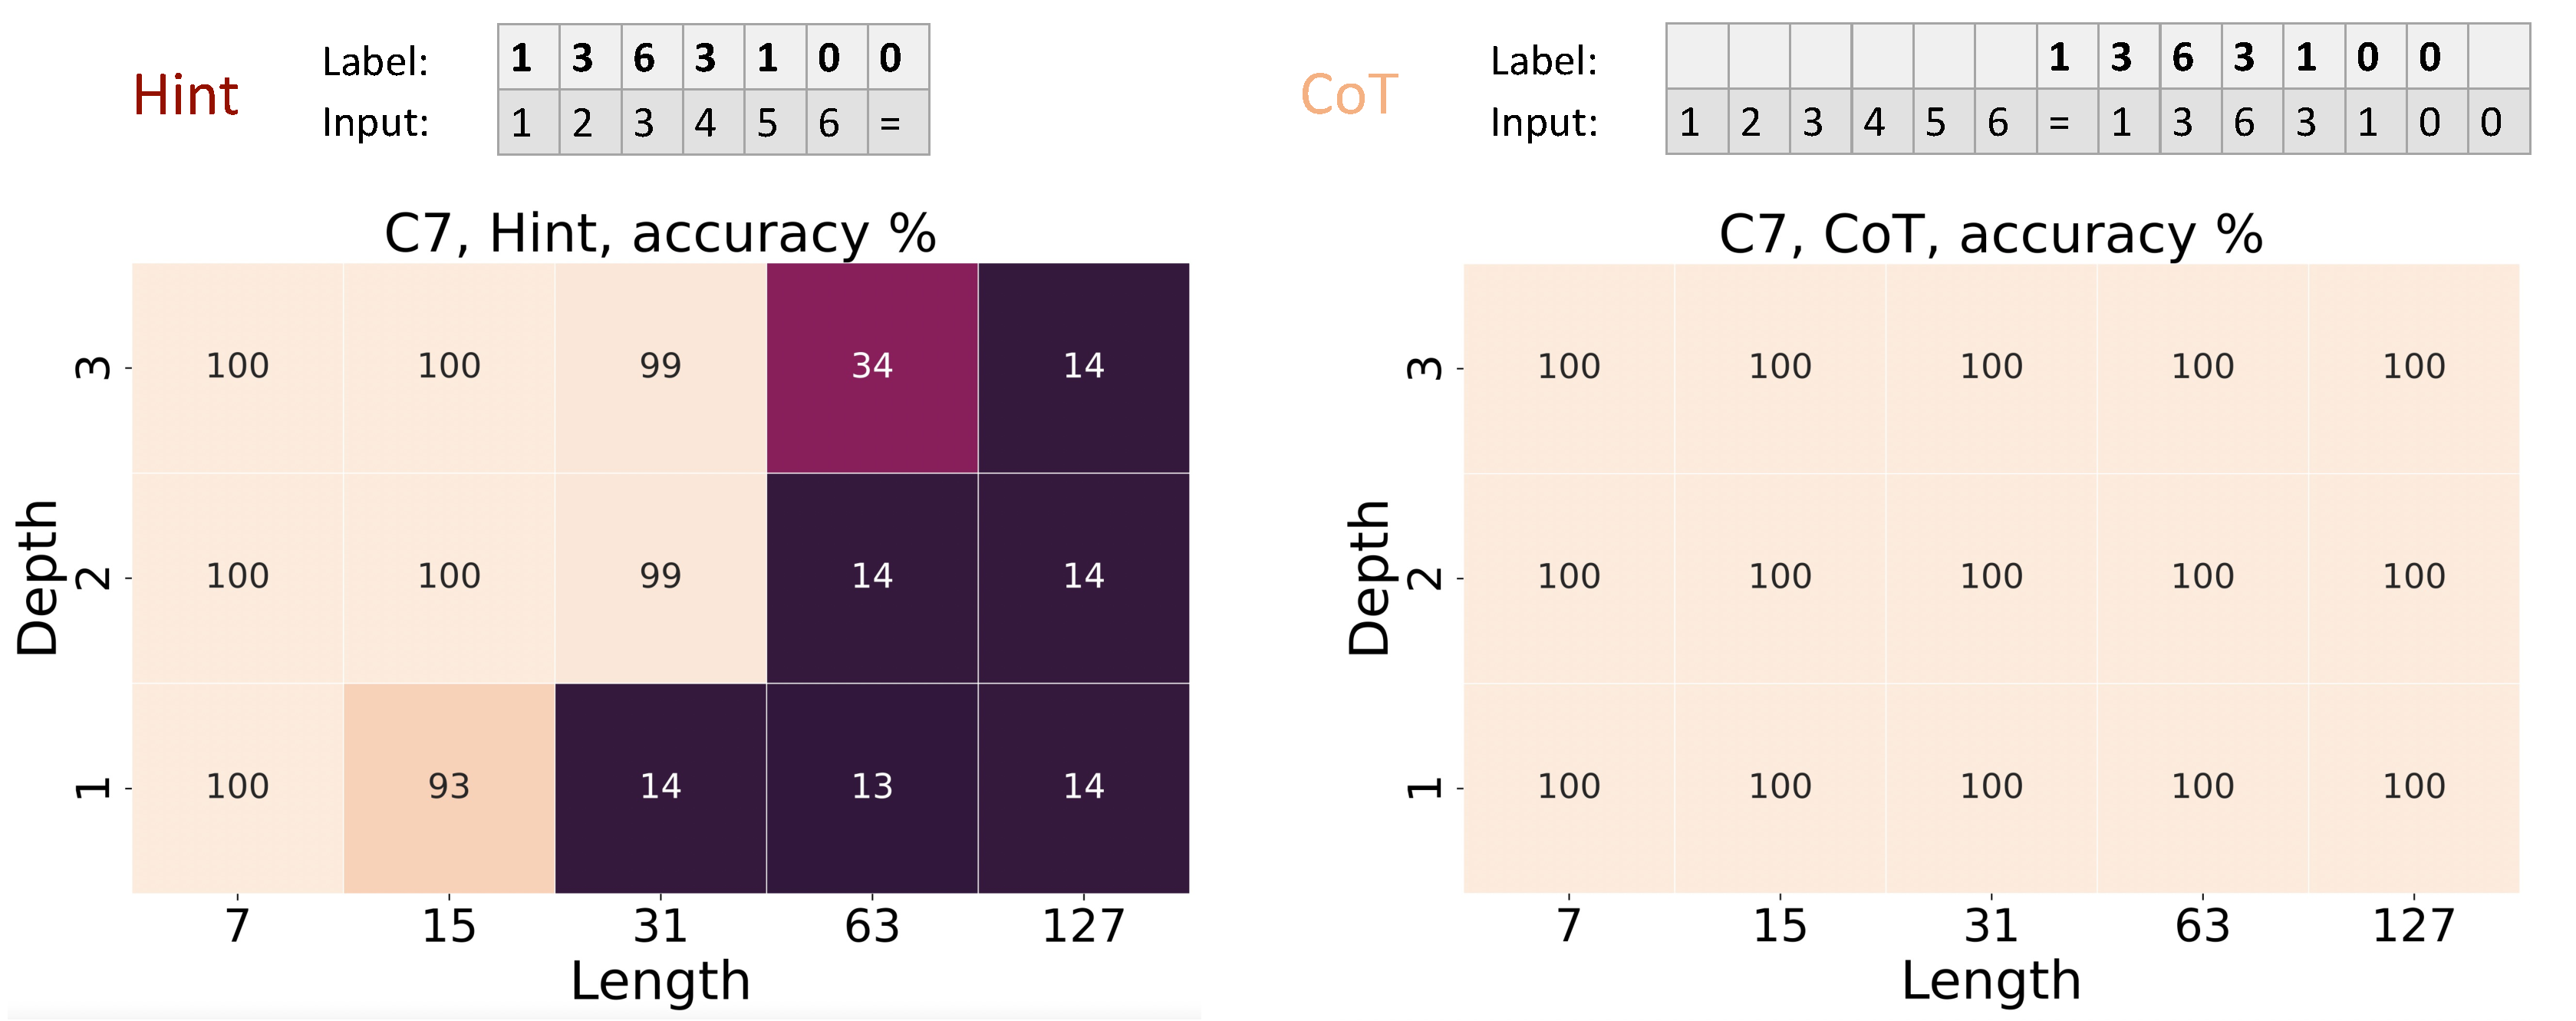
\includegraphics[width=0.96\textwidth]{figures/c7_iclr.pdf}
 
\caption{ Modular Addition($C_7$). The label is the sum of the inputs modulo a positive integer, which is $7$ in this case. The chain of thoughts and hints are the partial modular sum. Low-depth transformers with \hint\ can solve this task well for a reasonable input sequence length, but with \cot\ the performance is much better, especially with a long input sequence, as predicted by our \Cref{thm:cot_dlogn_main}. See experiments for $C_2$ in \Cref{fig:c2}.}  %\zhiyuan{edit the figure for arxiv}
 \label{fig:modular_addition}
\end{center}
 
\end{figure}

 
\section{CoT Empirically Improves Expressiveness of Low-Depth Transformers on Inherently Serial Problems}\label{sec:experiments}
 

This section is an empirical study of the expressiveness of decoder-only transformers with CoT on four different arithmetic problems: modular addition, permutation composition ($S_5$), iterated squaring, and circuit value problem. The first problem is parallelizable and can be solved by constant-depth transformers with log-precision while the latter three are inherently serial under some standard hardness assumptions in computational complexity or cryptography. As a prediction of our theory, we expect to see a huge improvement in accuracy when CoT is turned on.

\paragraph{General Setup.} 
To examine the expressiveness of decode-only transformers with and without CoT on these four types of problems, we train the transformer using $\Adam$~\citep{kingma2014adam} from random initialization in the online supervised setting for each problem and each different sequence length $n$. At each step, we sample a batch of training data from a distribution $p_n(x)$ where  $x= (x_1,\ldots,x_n)$ is training data and $y=f^*(x_1,\ldots,x_n)$ is the label. We always set $x_n$ to be '$=$'. We consider three different settings, \base, \cot, and  \hint:
\begin{itemize}
	\item \base: The optimization objective is simply $\loss_{\base}(\theta) \triangleq \Exp_{x\sim p}-\log p_\theta(f^*(x)\mid x)$.
	\item \cot: We manually design a chain of thought for each instance $x$, which is a string in $\gV$ and we denote by $c(x)$. We ensure the last token of $c(x)$ is always equal to the answer, $f^*(x)$. With $\tilde x\triangleq (x,c(x))$, the concatenation of $x$ and $c(x)$, and $m$ be the length of $c(x)$, the optimization objective is
	% \begin{align}
		$\loss_\cot(\theta)\triangleq \frac{1}{m}\Exp_{x\sim p}\sum\nolimits_{i=n}^{n+m-1} -\ln p_\theta(\tilde{x}_{i+1}\mid \tilde{x}_{1},\dots, \tilde{x}_{i})).$
	% \end{align}

	\item \hint: Even if the transformer has better performance in \cot\ setting than \base\ setting, one may argue that besides the difference expressiveness, \cot\ setting also has a statistical advantage over \base,  as \cot\ provides more labels and thus more information about the groundtruth $f^*$ to the model. This motivates us to design the following loss which provides the chain of thought $c(x)$ as the labels.
		Here for simplicity, we assume the length of $c(x)$ is equal to $n$. \footnote{Note such alignment is in general  impossible because the CoT $c(x)$ can be even longer than $x$ itself. However, in our four settings, there exist meaningful ways to set CoT $c(x)$ as hints for earlier tokens in $x$. } Formally we define  
		% \begin{align}
		$\loss_\hint(\theta)\triangleq \frac{1}{n}\Exp_{x\sim p}\sum\nolimits_{i=1}^{n}-\ln p_\theta(c_i(x)\mid {x}_{1},\dots, {x}_{i})).$	
		% \end{align}
\end{itemize}

 \begin{figure}[t]
 
\begin{center}
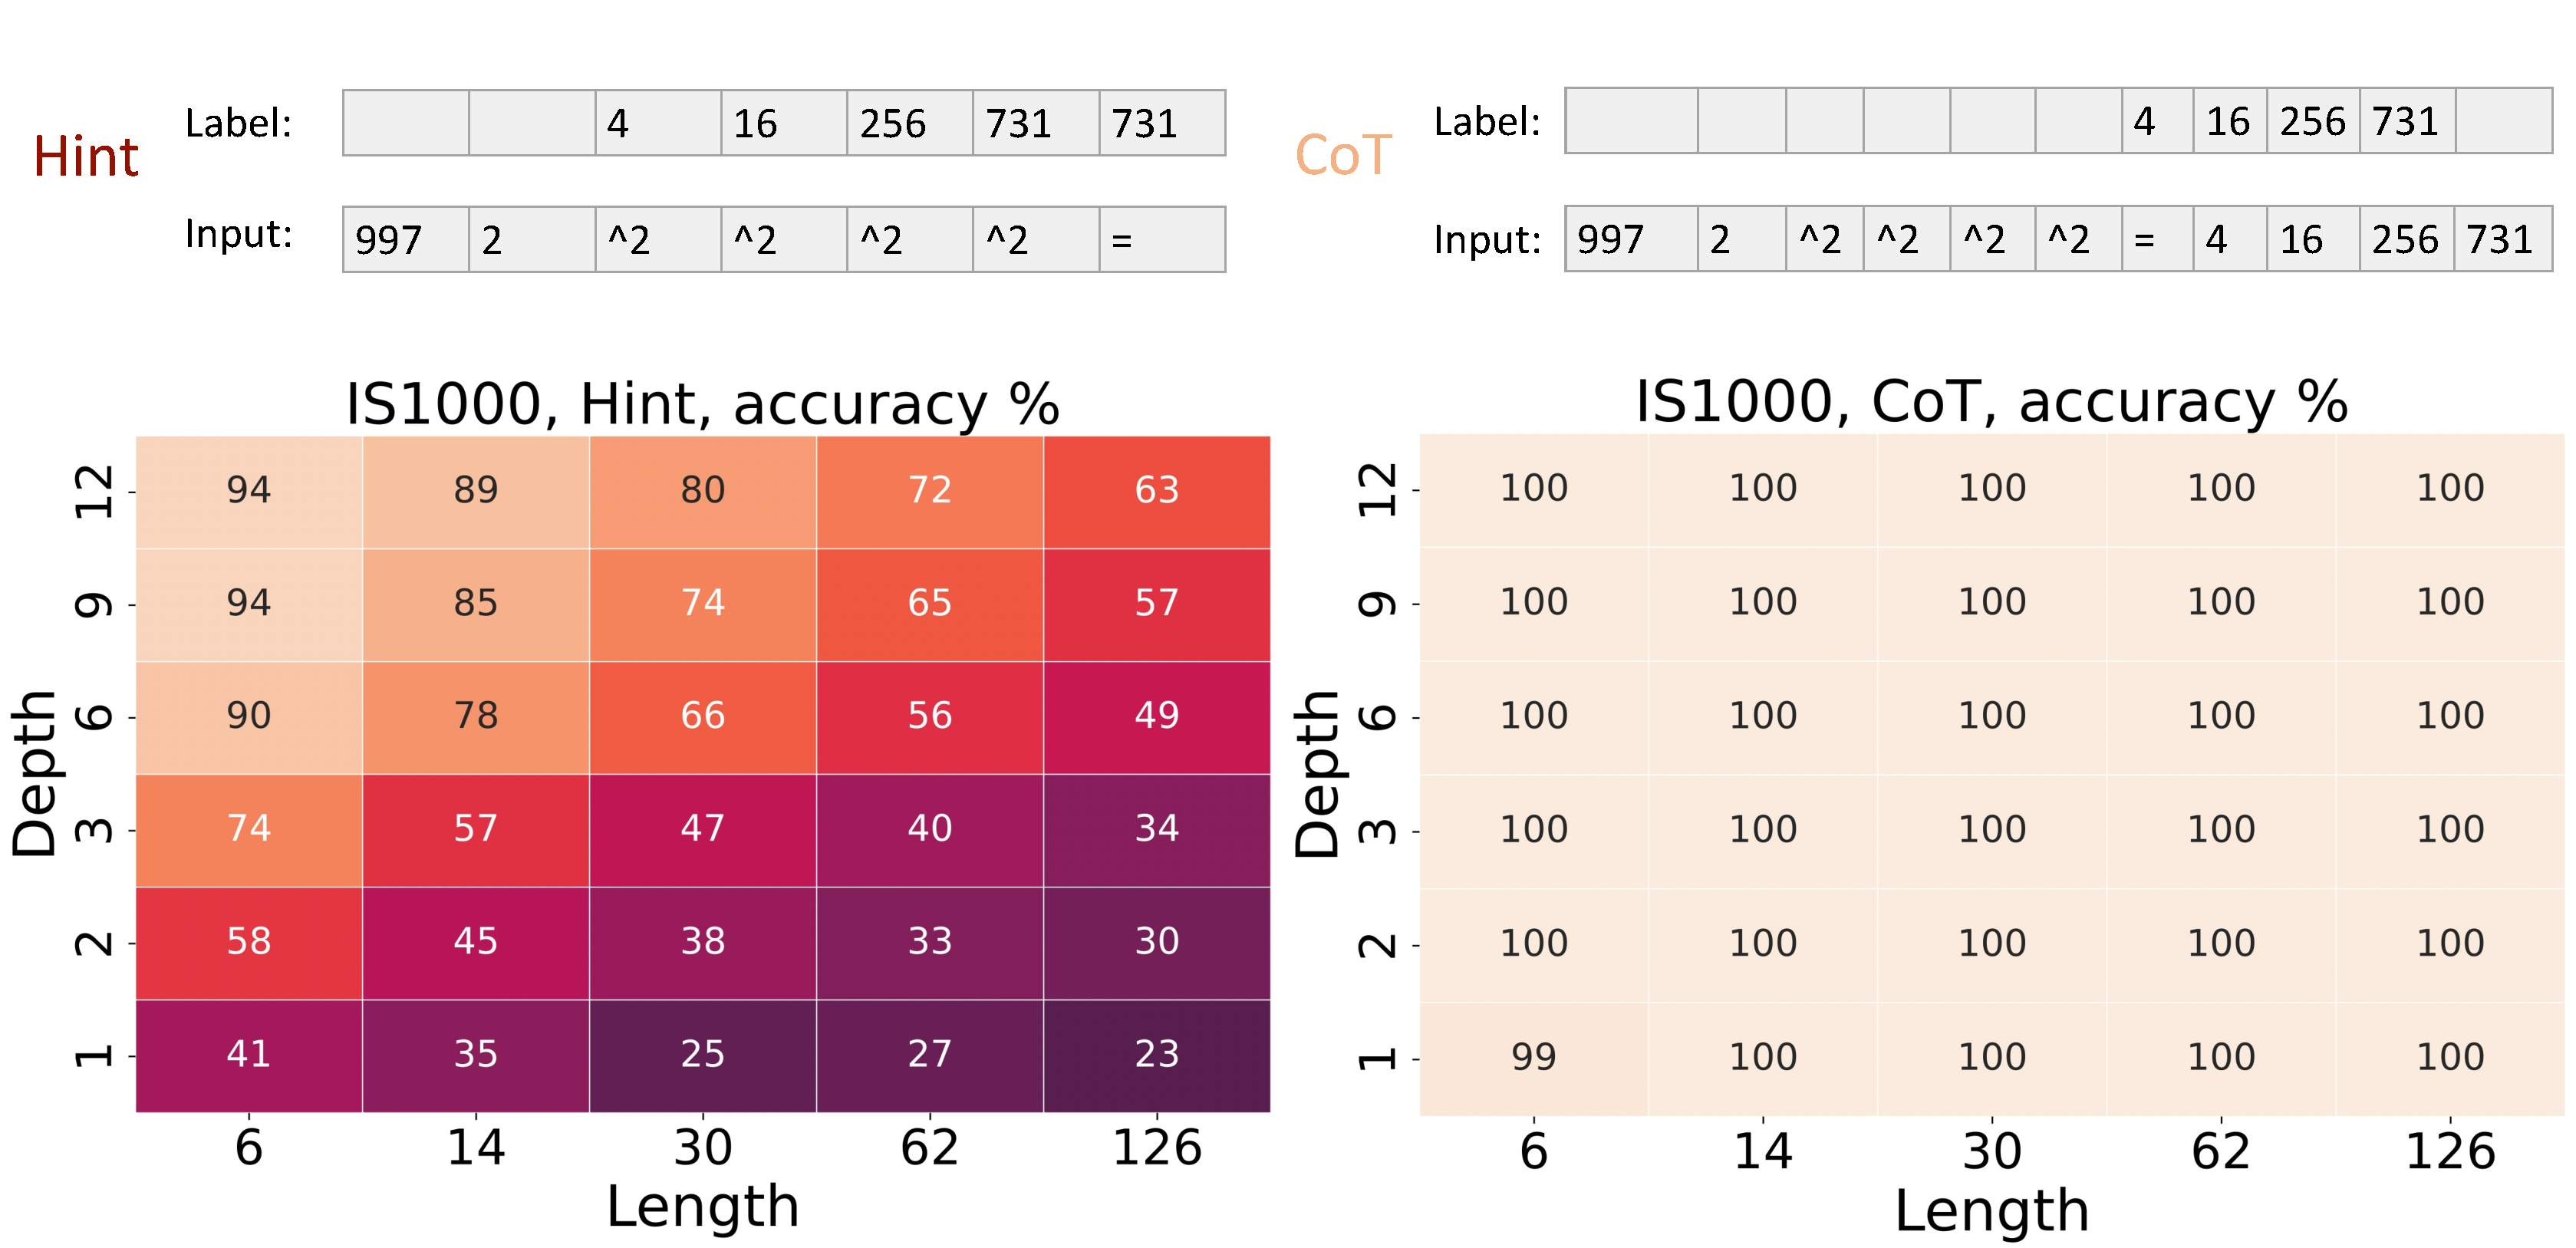
\includegraphics[width=0.96\textwidth]{figures/is1000.pdf}
 
\caption{\small Iterated Squaring(IS). The vocabulary  $\gV\triangleq\{0,1,\ldots,T-1,=, \text{\^{} 2}\}$ with $T=1000$. We randomly generate input of format  $(p,r, {\text{\^{} 2},\ldots,\text{\^{} 2}}, =)$ with $1\le r,p\le T-1$, $p$ being a prime and random number of \^{}2 tokens (at most $m$). 
The label is $f_{r,p}(n)\equiv (r^{2^n})\mod p$. CoT and hints are $(f_{r,p}(i))_{i=1}^n$. Though our construction does not exactly satisfy the technical conditions of the hardness assumption, this problem is difficult for  transformers without CoT to learn, but can be perfectly expressed with CoT even with depth  1.}\label{fig:iterated_square}
\end{center}
 
\end{figure}

\paragraph{Performance Evaluation.} Since we train transformers using fresh sampled synthetic data each step, the training accuracy/loss is just the same as validation accuracy/loss. For \base~and \hint~setting, we evaluate the accuracy of the final answer directly. For \cot~setting, directly evaluating the final answer is too easy because it only measures the ability of the transformer to correctly compute the last step since CoT is given as inputs. Ideally, we should measure the answer output by transformers after auto-regressively generating $|c(x)|$ tokens. But for computational efficiency, we measure the probability that transformers can predict all tokens in the given CoT correctly. Note this probability is a lower bound of the ideal metric because there is a small possibility that transformers can answer correctly with a wrong CoT. Nevertheless, even with this slightly more difficult evaluation metric, transformers in \cot~setting still optimize much faster than without CoT. 

Due to space limit, we defer the details of the training and each setting to \Cref{appsec:additional_exp}. Our experimental results are presented in \Cref{fig:modular_addition,fig:s5,fig:iterated_square,fig:cvp}.

\paragraph{Our Findings:} Unsurprisingly, the accuracy in \hint\ setting is always higher than \base\ setting. Due to the space limit, we postpone all results for \base\  settings into \Cref{appsec:additional_exp}. For the problems hard for parallel computation, \emph{i.e.}, permutation composition, iterated squaring, and circuit value problem, we find that \cot~is always better than \hint\ and \base, and the improvement is huge especially when depth is small. Our experiments suggest that turning on CoT drastically improves the expressiveness of low-depth transformers on problems that are hard to parallel compute, \emph{i.e.}, those inherently serial problems.  


\begin{figure}[t]
\begin{center}
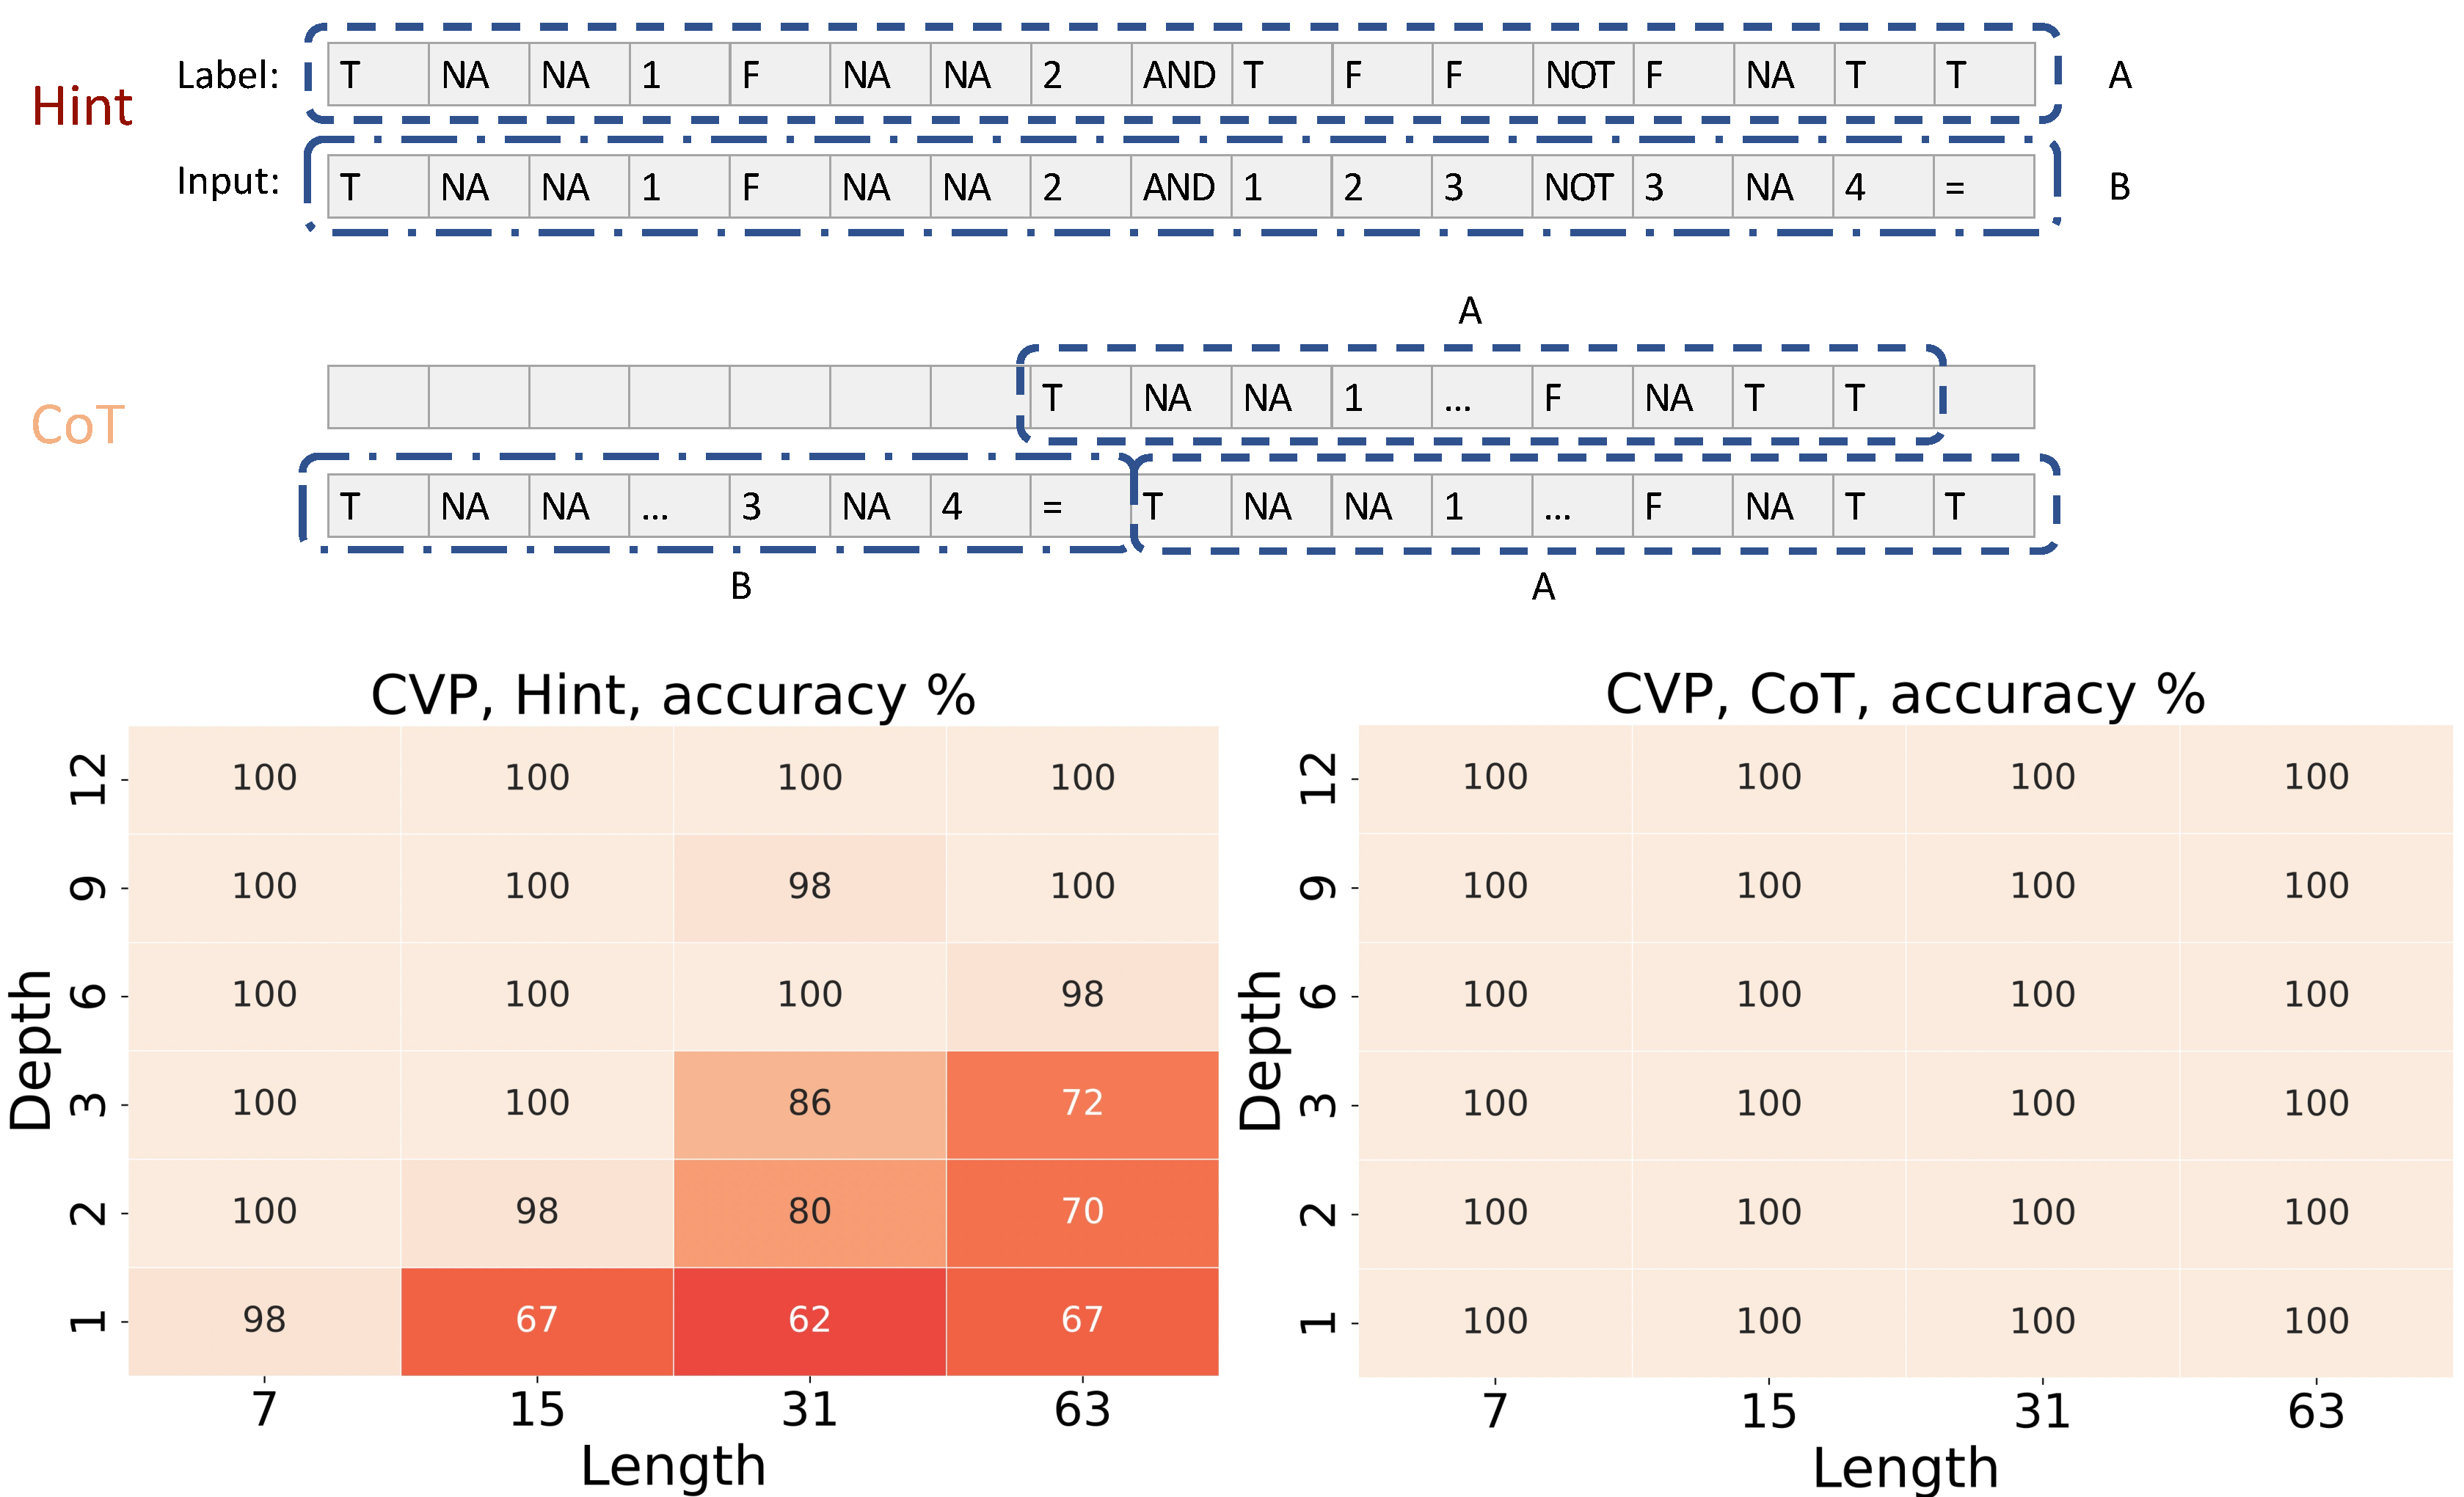
\includegraphics[width=0.96\textwidth]{figures/cvp.pdf}
 
\caption{Circuit Value Problem(CVP). Given a randomly generated circuit with $m$ gates (sorted by topological order), the vocabulary $\gV = [m]\cup \{ \True, \False, \AND, \OR, \NOT, \mathsf{NA}, = \}$. Each gate is represented by four consecutive tokens, which are gate type, two input gate ids, and  the current gate id. The output is the value of the last gate $m$. CoT and hints also contain 4 tokens for each gate, which are gate type,   two input gate values, and  the current gate value. 
 }\label{fig:cvp}
\end{center} 
\end{figure}

